\documentclass[12pt]{article}

\usepackage{amsmath}
\usepackage{mathtools}
\DeclarePairedDelimiter\ceil{\lceil}{\rceil}
\usepackage{mathtools}
\usepackage{algorithm}

\usepackage{algorithmic}

\usepackage{enumitem}

\usepackage{amssymb}
\usepackage{algorithmic}
\usepackage[ruled]{algorithm2e}

\usepackage{graphicx}

\usepackage{hyperref}
\usepackage[font=footnotesize]{caption}

\usepackage[utf8]{inputenc}
\title{ILWOA}
\begin{document}
\section{ILWOA}
    Cette version de l'algorithme utilise une fonction à dynamique chaotique et la distribution vol de Lévy afin de garantir une convergence rapide .Une phase de mutation est aussi rajoutée à la fin de chaque itération
\subsection{Fonction à dynamique chaotique}
Soit f:I $\rightarrow$ I une fonction continue.On suppose que la dynamique associée est chaotique.Alors:
\begin{enumerate}
    \item L'ensemble des points périodiques de f est partout dense dans I 
    \item f est sensible aux conditions initiales, ceci signifie que s'il y'a un petit changement dans la condition initiale $x_0$,le changement correspondant de $x_t=f_t(x_0)$ croit avec la croissance de t 
\end{enumerate}
Ce sont des fonctions qui permettent d'avoir une suite de nombres aléatoires qui dépend d'une condition initiale.Il existe plusieurs types de fonctions chaotique :fonction logistique,fonction de tchebychev.Après plusieurs tests, il a été remarqué qu'avec les fonctions logistiques nous obtenons une convergence plus rapide de la fonction objective .Le minimum de la fonction objective a été atteint en 5 itérations comme le montre le graphe(add refrence here)
\begin{figure}[h!]
   \centering
    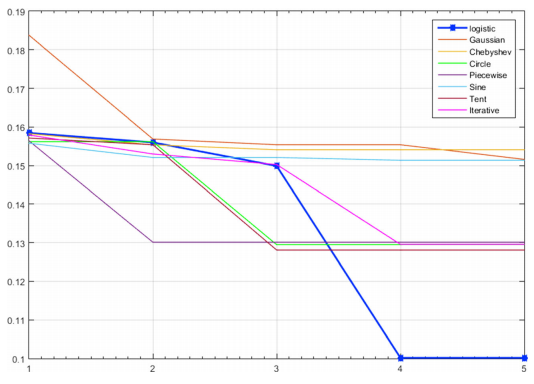
\includegraphics[width=10cm]{../figures/logisticvsothers.PNG}
    \caption[\small]{convergence fonctions chaotiques}
\end{figure}
Du graphe , on peut voir qu'avec la fonction logistique la fonction objective atteint le minimumu à partir de la 5eme itération
\subsubsection{Fonction logistique}
La fonction logistique est définie par la formule suivante :
\newline
\begin{center}
    $x_{n+1}=ax_n(1-x_n) ,x\in[0,1],0<a\leq4$   
\end{center}
où a est une constante caractéristique de la fonction logistique que nous avons fixé à la valeur give the value après plusieurs simulations
La fonction logistique est utilisée dans l'algorithme pour générer la valeur p
\subsection{La distribution vol de Lévy}
le vol de levy est un modèle mathématique caractérisé par une moyenne et une variance infinies ce qui rend le mouvement plus lent permettant ainsi une meilleure exploration de l'espace de recherche (REFERENCE).
Dans ILWOA , la variable C est remplacé par un pas aléatoire de la marche aleatoire levy donné par les formules suivantes:
\begin{align*}
&Levy\leadsto\frac{\lambda\Gamma(\lambda)\sin(\pi\lambda/2)}{\pi}\frac{1}{s^{1+\lambda}}\\
&s=\frac{U}{\left|{V^{\lambda^-1}}\right| },\quad U\leadsto N(0,\sigma_u^2),V\leadsto N(0,1)\\
&\sigma_u^2=[\frac{\Gamma(\lambda+1)}{\Gamma((\lambda+1)/2)}\frac{\sin(\pi\lambda/2)}{2^{(\lambda-1)/2}}]^{1/\lambda}
\end{align*}
\subsection{Phase de mutation}
Une phase de mutation a lieu à la fin de chaque itération.On vérifie d'abord si la solution atteinte est optimale .dans ce cas la recherche s'arrete sinon on applique la mutation sur cette dernière.
Cette phase est composée de 3 opérations exécutées séquentiellement comme le montre la figure (add fig number): 
\begin{itemize}
    \item Permutation: deux items de la solution sont choisis aléatoirement pour effectuer une permutation entre eux
    \item deplacement: Un sous ensemble d'items choisi aléatoirement est déplacé vers une position qui est egalement choisie aléatoirement
    \item Inversion: On applique une inversion sur un sous ensemble d'items
\end{itemize}
\begin{figure}[h!]
   \centering
    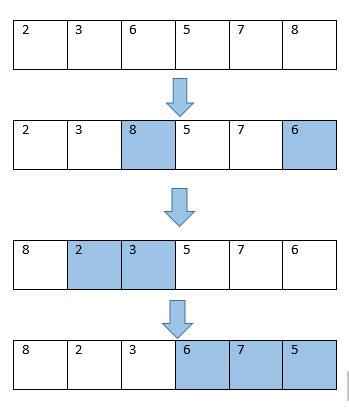
\includegraphics[width=10cm]{../figures/Mutation.PNG}
    \caption[\small]{Phase de mutation}
\end{figure}
\subsection{Pseudocode:}
\begin{algorithm}[H]
    \SetAlgoLined
    \KwResult{Nombre de boîte utilisées.}
    Initialiser la population de baleines (l'ensemble initial des solutions candidates): Xi (i = 1, 2 ,..., N)\;
    Évaluer les solutions de la population initiale\;
    X* = la meilleure solution actuelle\;
    \newline \While{\(t < max\_iter\)}{
        \For{solution \(\in\) population}{
            Mettre à jour a, A, C avec le vol de levy, l et p avec la fonction logistique\;
           \newline \eIf{\(r  < 0,5\)}{
                \eIf{\(|A| < 1\)}{
                    Mettre à jour la solution par Eq.(1)\;
                }{
                    Sélectionnez une solution aléatoire \(X_r\)\;
                    Mettre à jour la solution par Eq.(2)\;
                }
            }{
                Mettre à jour la solution par l'Eq.(3)\;
            }
        }
        Vérifier si une solution dans la population dépasse l'espace de recherche et la modifier\;
        \newline Appliquer la discretisation par LOV\;
        \newline Évaluer la nouvelle solution\;
        \newline Mettre à jour X* s'il existe une meilleure solution Sinon lancer la phase de mutation\;
        \newline Evaluer la nouvelle solution,màj de la meilleure solution
        t = t + 1\;
     }
    \caption{Improved Whale Optimization Algorithm}
    \end{algorithm}
\end{document}